\chapter{関連研究}
\label{related_works}

本研究が目指す「人馬一体」のような関係性は、、「身体化(embodiment)」の議論と関係が深い。

「身体化(embodiment)」は心理学や認知科学の領域で、Botvinick \& Cohen(1998)によるラバーハンド錯覚の報告を皮切りに「身体化感覚(sense of embodiment)」を中心として実証的知見が蓄積されている。本章ではまず、「身体化感覚」の概要と、他分野での応用や発展について、具体的な研究を紹介する。

\section{身体化感覚(sense of embodiment)}

身体化感覚は一般に、身体に対する所有感(sense of body ownership)、行為主体感(sense of agency)、そして自己位置感覚(sense of self-location)を合わせた感覚として取り扱われる\cite{kilteni2012}。その元となったのは、Gallagherの「ミニマルセルフ」という概念である。「ミニマルセルフ」とは、自我としてみなしうる必要最小限のもののことであり、身体所有感(sense of ownership)、行為主体感(sense of agency)の二つから構成されていると説明される\cite{Gallagher2000}。

こうした自己についての説明を実験的に操作・検証可能としたのがBotvinick
\& Cohenによるラバーハンド錯覚\cite{BotvinickCohen1998}である。これは、自分の手を衝立の裏に隠し、偽物の手を目の前に置いた状態で、両方に同じタイミングで刺激を提示すると、偽物の手を自分の手であるように感じる錯覚である。この報告により、外界の対象への身体所有感の生起が可能であることが示されたとともに、身体所有感研究に関する系統的な手法が開発されることとなった。

そしてこの知見は、VR、ロボティクス、インターフェースデザインなどの領域での応用や、更なる基盤技術の開発へと発展している。

\section{VRにおける身体化感覚}

近藤ら\cite{Kondo2020}は、右手の親指の動きにVR上の左腕の動きを連動させることで錯覚的な身体所有感(Illusory Ownership)が生じるのかについて検証した。被験者は、右手の親指の動きがVR上での左腕の動きにマッピングされている様子をヘッドマウントディスプレイを介して確認する。実験では、被験者に5分間自由に指先を動かしてもらった後、VR上で左腕のあたりにナイフが突然出現する。このときの皮膚電導反応(Skin Conductance Response, SCR)の計測と、身体化感覚(embodiment)に関するアンケートを20人の被験者に行った結果、この手法を通して右手の親指と左腕の結びつき(re-association)は、程度は弱いが誘発できると報告している。

また佐々木ら\cite{sasaki2022multisoma}は、VR上で最大4つの身体を制御できるシステムを実装し、複数の身体を制御する際、人間の身体認知がいかに更新されるかについて検討した。実験では3つのタスクを設定し、視線情報、タスクのパフォーマンス、身体化感覚(sense of embodiment)についての主観評価により、これらの身体の認知を評価した。結果、人間は複数の身体を同時に操作することで、それぞれの身体に対して身体所有感(sense of ownership)や運動主体感(sense of agency)を持つことができると報告している。

\section{ロボティクスにおける身体化感覚}

Kielibaら\cite{kieliba2021robotic}は、ロボットで拡張された親指が人間の運動能力を拡張させることができるかどうか、そしてそれが手の神経表現や機能にどのような影響を与えるのかを調査するため、The Third Thumbというロボットの親指を用いた研究を行った。この親指は、足のつま先で操作することができる。
5人の参加者は、5日間にわたってThe Third Thumbを装着し、実験室での使用と日常生活での使用が求められた。通常は両手を使って行うタスクをこの親指を駆使して片手で行い、その器用さ(dexterity)や身体化感覚(sense of embodiment)などの度合いが評価された。トレーニングを経て、認知的負荷が増加した場合や視覚が遮断された場合でも、親指の運動制御、器用さ、そしてThe Third Thumbに対する身体化感覚(sense of embodiment)が向上したと報告している。

\section{インターフェースデザインにおける身体化感覚}
インターフェース研究者の渡邊は、ユーザインターフェースにおける「透明性」を実現する上で「自己帰属感(sense of ownership)」に着目した\cite{Watanabe2017}。
ここで「透明性」とは、道具の使用において、使っている最中にはその道具自体を意識せずに身体の一部になったかのようになり、目的に集中できるようにすることとされている。

そして、道具の透明性は「自己帰属感」によってもたらされると考え、マウスカーソルを対象に、ユーザインターフェースにおける自己帰属感を検証する「ダミーカーソル実験」を行った\cite{Watanabe2013}。この実験ではスクリーン上に、マウスと連動して動く通常のカーソ
ルの他に色形状の同じの複数のダミーのカーソルをランダムに動くように同時に提示する。被験者は動きのみでしか自身のカーソルを判別することができない環境になる。そしてこの実験によって、人は動きのみであっても複数のダミーカーソルの中から自身のカーソルを発見できると報告されている。どれが自分のカーソルか判別できることから、人間はカーソルに対しても自己を見出しており、自己帰属感が生起していると主張している。
これを踏まえて、ユーザインターフェースにおける自己帰属感を生起するために、操作時の動作とグラフィックの追従性が重要となることを指摘した。

\section{本研究の位置付け}
ここまで概観したように、「身体化感覚」をキーワードとしてその可能性や限界を探る研究が発展してきた。特に、VR分野での身体化研究は、身体全体の大きさや数など、扱える操作変数が多いため、新しい心理学研究の可能性を拓いていると言える。
また、インターフェースデザインにおいては「使いやすさ」や「直感性」を身体化の枠組みから捉え、応用されるなど、人と道具、機械などの関係性の設計を考える上でも重要なテーマと言える。

しかしその一方で、本研究が着目するような、身体化するまでの過程における主観的な体験に関する研究が不足している。

ここで「身体化の過程」に注目すると、結果としては同じ身体化であっても、そこには質的な違いが存在することがわかる。例えばラバーハンド錯覚とThe Third Thumbは、いずれも身体化感覚が生起している点では共通する。しかし、前者は受動的な触覚提示によっても身体化が生じているのに対し、後者の身体化は「器用さ(dexterity)」を途中で獲得することで身体化が生じる。その過程では「もどかしさ」や「楽しさ」を経験すると考えられる。つまり、身体化するまでの意識的な試行期間の有無という点において異なっている。

% アバターに対して様々な介入が可能なVR分野では、身体拡張における可能性や限界を探る上で格好のフィールドであると言え、佐々木らや近藤らによる研究は、身体化感覚を評価軸とした様々な身体操作を実現するための基盤技術の研究であると位置付けられる。

% 一方Kielibaら\cite{kieliba2021robotic}の研究は、拡張された身体部位との協調(human-hand cooporation)が芽生えるまでの5日間という比較的長い調査期間を設け、身体化感覚の変化に着目している点で特徴的である。

そのため本研究は、身体化の過程での経験をより細かく説明するために、一般に用いられる「身体化感覚(sense of embodiment)」ではなく、コンピュータ工学研究者のSydney Felsによる身体化の程度についての分類を援用する。Felsは、人が対象に対してどのような感情を抱いているかに注目することで、「身体化」の程度を捉えた。これにより、身体化に関する新たな方向性を捉えることができるのではないかと考えた。

% \section{身体化感覚(sense of embodiment)との相違}
% 「Embodiment」という言葉は心理学研究やHCI分野において、一般には身体化感覚(sense of embodiment)を言及する意味において使用される。これは、身体に対する所有感(sense of body ownership)、行為主体感(sense of agency)、そして自己位置感覚(sense of self-location)を合わせた感覚として取り扱うことが多い\cite{kilteni2012}。
% この概念は「人間がいかに現実を認識しているか」を理解することで技術を発展させてきたバーチャル・リアリティ(VR)分野において実験的に操作・検証可能とするために整理されたものであるが、その元となったのは、Gallagherの「ミニマルセルフ」という概念である。

% 「ミニマルセルフ」とは、一切の自己知識を失ったとしても残る最小限の自己であり、身体所有感(sense of ownership, body ownership)、行為主体感(sense of agency)の二つによって支えられていると説明される\cite{Gallagher2000}。

% こうしたGallagherの説明を起点にそれらを評価する方法が考案され、ラバーハンド錯覚実験などにみられるように、生来の肉体ではないものを自分の身体と錯覚してしまうような人間の身体像の曖昧さに注目した研究が認知科学や心理学の領域で取り組まれてきた\cite{braun2018senses}。こうした研究で蓄積された実証的知見は、インターフェースデザインや身体拡張の設計・評価へと応用されている。渡邊がマウスカーソルやスマートフォンの道具としての透明性を説明する上で用いた「自己帰属感」も、Gallagherの「sense of ownership」に対する訳語である\cite{Watanabe2017}。

% しかし、この意味でのembodimentは、「人間の一部として対象が帰属しているような状態」についてのみ言及するものである。embodimentは日本語で「身体化、一体化、身体性」などと訳されるが、動詞の「embody」についてCambridge Dictionaryで引くと、
% \begin{quote}
%   \begin{enumerate}
%     \item \textit{to represent a quality or an idea exactly} (質や考えを的確に表すこと) 
%     \item \textit{to include as part of something} ((何かを)何かの一部として取り込むこと)
%   \end{enumerate}
% \end{quote}
% とある\cite{embody}。ここで指摘したいのは、2つ目の意味からembodimentの原義とは「何かを取り込んで、何かの一部とすること」であり、「人間の一部として対象が帰属しているような状態」のみを指すわけではないということだ。

% \section{身体の変換や拡張の試み}
% 身体の変換や拡張といったテーマは、embodimentの理論を踏まえて近年様々な研究が行われている。
% % 高度化・複雑化する技術が高い表現力や能力を持っていたとしても、それを扱う人間の能力が追いつかない限り、有効活用することができない。この問題は、群ロボット制御のような人間の身体性を越えた技術、そして身体の変換や拡張に取り組む分野で顕著に現れる。

% % Kimらは、複数台の卓上ロボット群を効果的に制御するための、インタラクション様式のセットと、そのデザインガイドラインを提示した。複数台で連携を取り合いながら、柔軟に役割を変えて複雑なタスクを達成することのできる群ロボットには、個々のロボットが持つ能力の総和以上の可能性がある一方で、それらを効果的に操作するためのインタラクション様式の設計に関する研究は少ない。そこで、卓上ロボット群に達成してほしいタスクを伝えられた被験者が、実際に卓上ロボットを前にしたとき、どのような働きかけをしてそれらを動かそうとするのかを観察することで、自然なユーザの動きを引き出すという手法(Elicitation Study)によって、様々なシチュエーションに対する適当なインタラクション様式を示した。

% % 稲見らによる自在化身体プロジェクト\cite{jizai}では、人間がロボットや人工知能などと「人機一体」となり、自己主体感を保持したまま自在に行動することを支援する「自在化技術」の開発と、「自在化身体」がもたらす認知心理および神経機構の解析をテーマにウェアラブル技術やバーチャル環境における共有身体の操作における基盤技術の開発に取り組む。
% 近藤らは、右手の親指の動きにVR上の左腕の動きを連動させることで錯覚的な身体所有感(Illusory Ownership)が生じるのかについての検証を、20人の被験者を対象に行なった\cite{Kondo2020}。モーショントラッキングを用いて取得された右手の親指の動きがVR上での左腕の動きにマッピングされている様子を、被験者はヘッドマウントディスプレイを介して確認する。実験では、5分間自由に指先を動かしてもらった後、VR上で左腕のあたりにナイフが突然出現する。このときの皮膚電導反応(Skin Conductance Response, SCR)の計測と、一体化(embodiment)に関するアンケートの結果から、この手法で錯覚的な身体所有感は確実に誘発できるものの、その程度は弱いと報告している。

% また佐々木らは、VR上で最大4つの身体を制御できるシステムを実装し、複数の身体を制御する際、人間の身体認知がいかに更新されるかについて検討した。実験では3つのタスクを設定し、視線情報、タスクのパフォーマンス、主観評価により、これらの身体の認知を評価した。結果、人間は複数の身体を同時に操作することで、それぞれの身体に対して身体所有感(sense of ownership)や運動主体感(sense of agency)を持つことができることがわかった。\cite{sasaki2022multisoma}。

% これらの研究は、親指の動きで動く左肩や複数の身体など、自分の肉体とは異なる身体ではあるが、それを自分の身体であるかのように認知しやすいものとそうでないものとの境界を探っていくこと、ひいては人間の認知的特性の理解に関心があると捉えられる。

% 一方で、次に紹介するKielibaらの研究は、同じく身体性(embodiment)についての評価が含まれるが、変換された身体のもとで行動する期間が長く、時間を経て身体性が獲得されることについて取り組んでいる。

% % 身体の変換や拡張を行う研究は近年、数多く行われている\footnote{近年に多いとする根拠は、小鷹の「ラバーハンド錯覚の遅い発見問題」という問題意識に基づく。小鷹は、「ラバーハンド錯覚」というシンプルな錯覚が学術的にはじめて発表されたのが1998年と遅く、それが「コンピュータの普及により、事物を情報的に処理する感受性が世界に浸透しつつあった1990年代後半」であったことに、単なる偶然ではない「情報としての身体」という発想を後押しするものがあったのではないかと指摘する\cite{kodaka}。}\cite{Kondo2020, ekusute,Kasahara2017,augmented_hand_series}。そうした実践の中心的な関心について、ここでは「錯覚」と「身体に対する再注目」であるとして、先行事例を紹介する。その上で、それぞれの関心と本研究の関心の相違点を説明することで、研究の位置付けを明らかにする。

% % しかし本研究の関心は「錯覚」ではない。そうではなく、突然自分の体とは似ても似つかない、それでいて扱い方もわからないような身体を与えられたときに、どう一体化していくかということに関心がある。

% % 小川らによる「えくす手(Metamorphosis Hand)」\cite{ekusute}では、指の伸びた手などの現実の身体にはあり得ない特性を持ったバーチャルな身体を通じてピアノを演奏することができる。そのねらいは、「現実とは異なる特性のバーチャルハンドへの身体所有感の生起を通じ、現実の身体的制約を超えたインタラクションを実現する、一種のバーチャルな身体拡張体験を提供する」と説明される。

% Kielibaら\cite{kieliba2021robotic}は、ロボットで拡張された親指が人間の運動能力を拡張させることができるかどうか、そしてそれが手の神経表現や機能にどのような影響を与えるのかを調査するため、The Third Thumbというロボットの親指を用いた研究を行った。この親指は、足のつま先を用いて操作することができる。
% 5人の参加者には、5日間にわたってThe Third Thumbを装着した状態で通常は両手を使って行うタスクを、この親指を駆使して片手で行い、その器用さ(dexterity)や身体性(sense of embodiment)などの度合いが評価された。トレーニングを経て、認知的負荷が増加した場合や視覚が遮断された場合でも、親指の運動制御、器用さ、そしてThe Third Thumbとの協調性が向上した。

% Kielibaらの研究では、体験者は身体が変換された状態を比較的長い期間経験し、参加者が特殊な能力を獲得していくことについての時間的変化を扱っている。これは近藤らや佐々木らの研究とは違い、身体の拡張の試みの中でも、人間の能力の獲得に関心があると捉えられる。こうした人間の能力の獲得の過程には、FelsのいうBelongingの意味での一体感(embodiment)が見られる。

% 本研究が身体の変換表現に取り組む理由は、後者のKielibaらの研究に見られる関心と共通している。つまり人間が自分の身体とは程遠い変換に対して、どのようにその扱い方を見出していくのかに関心がある。そのため本研究の中で探求する身体の変換表現においては、生来的に備わっている認知的特性によって一体感を得るのではなく、人間が意識的に注意を向けて体験することで一体感を得ることが重要である。

% ただし、本研究において取り組む変換の表現は、Kielibaらほど一体感を経験するまで長い期間を要するものではない。だが、短い期間であるからこそ人間が注意を向けている間の経験について、詳細に記述することが可能である。これらを踏まえると本研究の貢献とは、次章で説明する\textit{grasp}の概念を用いて、Intimacyが生じるまでの過程についての詳細な説明を可能にすることである。

% 身体所有感の生起要因に関するこれまでの議論を参照し、本作は「テクスチャ、形状、空間的配置、解剖学的構造の4つの特性」を根拠に、身体所有感が生じながらも、自己身体と意味的に類似しないバーチャルハンドを制作している。これらの特性は、身体所有感を生じさせる上での実証的知見ではあるが、本研究が対象とするIntimacyは、例えば楽器のように、こうした生起要因を押さえなくとも、習得を経て生じうるのではないかと考える。また、生起要因を多く踏襲しているわけではないからこそ、身体所有感が生じるまでには期間を必要とし、その程度にも個人差が生じるのではないだろうか。これらの観点から、本研究の取り組みは「えくす手」よりも極端な身体変容を促す体験として位置付けられる。

% \subsection{身体に対する再注目}
% Golan Levinらによる《Augmented Hand Series》\cite{augmented_hand_series}は、ウェブカメラによって取得した体験者の手の映像をリアルタイムに変形し、指の本数や長さなどの異なる手を投影する作品である。また、佐藤雅彦らによる「君の身体を変換してみよ展」では、さまざまなアプローチで身体の変容を扱う作品が展示されたが、その中でも《点にんげん・線にんげん》\cite{sato_icc}という作品では、動物の関節などの位置を示す点の動きだけでも脳が「生物的な動き」としてひとまとめに認識できる(バイオロジカルモーション)という現象を活用し、体験者の関節の位置が表示された点群が、様々な方法で結びつけられたり、ある役割を与えられるなどの「変換」に対して、「自分の身体である」という認識が保たれたまま形が変わっていく作品である。

% これらの作品の関心は、「身体に対する再注目」であると考えた。いずれも、身体が異なる見た目に変わったというだけであって、実用的な特別な能力が付与されたり、ゲーム性があるわけではない。それでも身体を動かしてみることの動機は、「動くこと」そのものへの興味が働いているからである。これは、生後まもない乳児が自分の手の存在に気づき、手を見つめたり、動かしたりしながらよく観察する動作である「ハンドリガード」に似た現象であると解釈した。「身体の変換」を通して、新しい身体像を得たことから生じた「注目」と向き合う契機となる。

% こうした関心の作品を、ここでは生まれ持った肉体に対する「注目」を最初と数えて、「身体に対する再注目」とした。

本章では、本研究における「人馬一体」といった関係性についてより詳細に捉えるため、Sydney Felsによるembodimentの分類を導入する。
そして、そのような一体感が生じる上で重要であると考える\textit{grasp}と言う概念を、新たに提示する。

\section{Felsのembodiment}
コンピューター工学の研究者であるSydney Felsは2000年、「Intimacy and Embodiment: Implications for Art and Technology」\cite{Fels}において、人間と対象との関係性を「embodiment」の観点から4つのカテゴリに分類した。
それぞれの説明は以下の通りである(括弧内は筆者訳)。

\textbf{Response(応答):}\\
対象に対する作用の結果から、感情的な反応や理解を得る状態を指す。Felsはこの関係性の例として「コンピュータとそれに初めて触れた人」を挙げ、「なんらかの操作を通して得られた、便利な機能に喜んでいる状態、また逆に「有用な結果を得られず落胆する状態」と説明する。

\textbf{Control(制御):}\\
人が対象を自分自身の延長として使用し、その操作によって感情的な満足や美的体験を得る状態を指す。例えばピアノの演奏において、「音が出ている」ということだけでなく、自分自身の表現したいことが、不自由なくピアノを通して体現されていると感じるときの、一体感によってもたらされる心地よさがこれに該当する\footnote{「Control」においてFelsは、「自分自身の延長」として経験される感覚であり、またそれが追従性の高いグラフィックによってもたらされると説明する。これは、渡邊がマウスカーソルやスマートフォンに対して用いた「操作時の指とグラフィックの追従性が高い」インターフェースという説明と同等のものであると考えられる。このことからFelsの分類におけるControlは、渡邊の「自己帰属感」と重なる。}。

\textbf{Contemplation(鑑賞):}\\
人が対象に対して働きかけることはないが、人がその対象からの信号やメッセージを内省や反映を通じて、感情的になったり美的体験を得る状態を指す。Felsはその具体例として、絵画の鑑賞体験を挙げる。

\textbf{Belonging(帰属):}\\
対象によって人が動かされているような経験を指す。人はその対象によって提供される体験を通じて感情的な反応を得る。ここでは、対象が人の体験や感情を形作る役割を果たす。たとえばバイクの運転において、「バイクに合わせた走り方をする」といったように、単にその対象を通して使い手の意図がそのまま体現されるのではなく、その対象に合わせた振る舞いがそこで形作られることに喜びを見出すような状態である。

\begin{figure}[H]
  \centering
  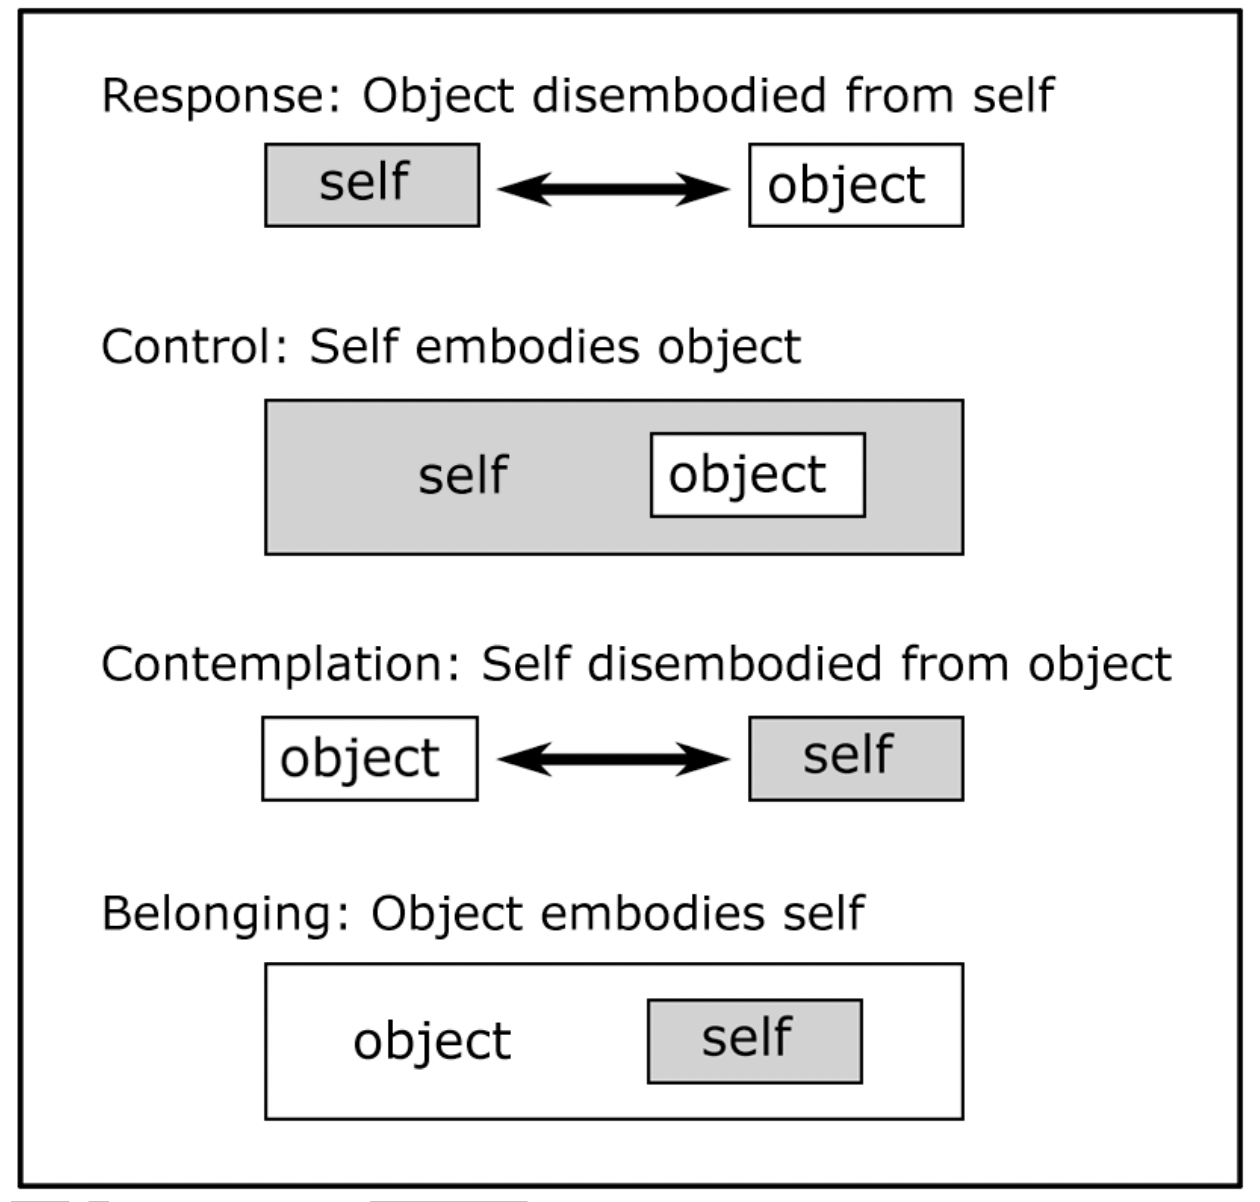
\includegraphics[width=8cm]{img/fels_diagram.png}
  \caption{Felsによるembodiment(仮置き)}
  \label{fig:fels_embodiment}
\end{figure}

% さて、Felsは特に、上記「制御 Control」においては「自分自身の延長」として経験される感覚について言及しており、またそれが追従性の高いグラフィックによってもたらされるという記述は、渡邊がマウスカーソルやスマートフォンに対して用いた「操作時の指とグラフィックの追従性が高い」インターフェースという説明と同等のものである。このことからFelsのいうControlとは、Gallagherの「sense of ownership」と同じものを指していると考えられる。その上で、embodimentの状態をControlのみならずBelongingから捉えていること、そしてembodimentが生じていない状態についても言及していることなど、現在HCIの分野で一般に用いられる意味でのembodimentよりも広く、人と対象を捉えるモデルとなっていることが確認できる。

% さらにFelsは、対象と人とのあいだにある「深い関係」を指して、「Intimacy」という尺度で説明する。例えば楽器と人の関係性ように、Intimacyのある関係性のもとでは、「あたかもその装置が身体の延長であるかのように、考えや感情を効果的に表現できる」という。上記の、Felsによるembodimentの分類においては、ResponseがIntimacyの低い状態、ControlがIntimacyの高い状態として説明される。
